\chapter{Biological Background}
    \label{cha:biologicalBackground}
    %
    %
    % MOLECULE DEFINITIONS -- START
    \definesubmol{lysine}{
        % 1
    R-[:330,0.7]\mcfbelow{N}{H}% 2
    -[:30,0.7]% 3
        (
    -[:330,0.7]% 4
            (
        =[:270,0.5]O% 6
            )
    -[:30,0.7]R'% 5
        )
        (
    <:[:50,0.7]H% 8
        )
    <[:110,0.7]% 7
    -[:30,0.7]% 9
    -[:330,0.7]% 10
    -[:30,0.7]% 11
    -[:330,.5,,1]NH_3^{\mcfplus}% 12
    }

    \definesubmol{acetylcoa}{
            % 1
        CoA-[:330,0.7]S% 2
        -[:30,0.7]% 3
                (
            =[:90,0.5,,,red]{\color{red}O}% 5
                )
        -[:330,0.7,,,red]% 4
    }

    \definesubmol{acetyllysine}{
            % 1
        R-[:330,0.7]\mcfbelow{N}{H}% 2
        -[:30,0.7]% 3
                (
            -[:330,0.7]% 4
                    (
                =[:270,0.5]O% 6
                    )
            -[:30,0.7]R'% 5
                )
                (
            <:[:50,0.7]H% 8
                )
        <[:110,0.7]% 7
        -[:30,0.7]% 9
        -[:330,0.7]% 10
        -[:30,0.7]% 11
        -[:330,0.7]\mcfbelow{N}{H}% 12
        -[:30,0.7]% 13
                (
            -[:330,0.7,,,red]% 15
                )
        =[:90,0.7,,,red]{\color{red}O}% 14
    }
    % MOLECULE DEFINITIONS -- END
    %
    % \section{Epigenetics}
    % general and historic (very short or leave out)\\
    % instructive, responsive model\\
    % PCG Tri\\
    %
    %
    % \section{Eukaryotic transcription regulation}
    %
    \section{Chromatin}
        %
        Each of the three domains of life features chromosomal architectural proteins (ChAPs) which interact with DNA and play a major role in its spatial organization in order to ensure efficient replication, segregation and gene expression \cite{prohaska2010innovation}. The most well-researched proteins among ChAPs are histones consisting of a dimerized helix-loop-helix-loop-helix motif \cite{selleck2001histone}.
        %

        %
        While all major archaeal lineages feature histone tetramers \cite{slesarev1998evidence}, eukaryotic chromatin consists of DNA which is wrapped around histone octamers to form so-called nucleosomes. Except for Dinoflagellates which feature a different type of ChAPs \cite{de2005organization}, histones are evolutionarily conserved throughout all eukaryotic organisms. Interestingly, Bacteria completely lack histone homologues. Instead, they feature a different group of architectural proteins, called nucleoid-associated proteins (NAPs) \cite{qin2019architects}.
        %

        %
        \begin{figure}[htpb!]
            \centering
            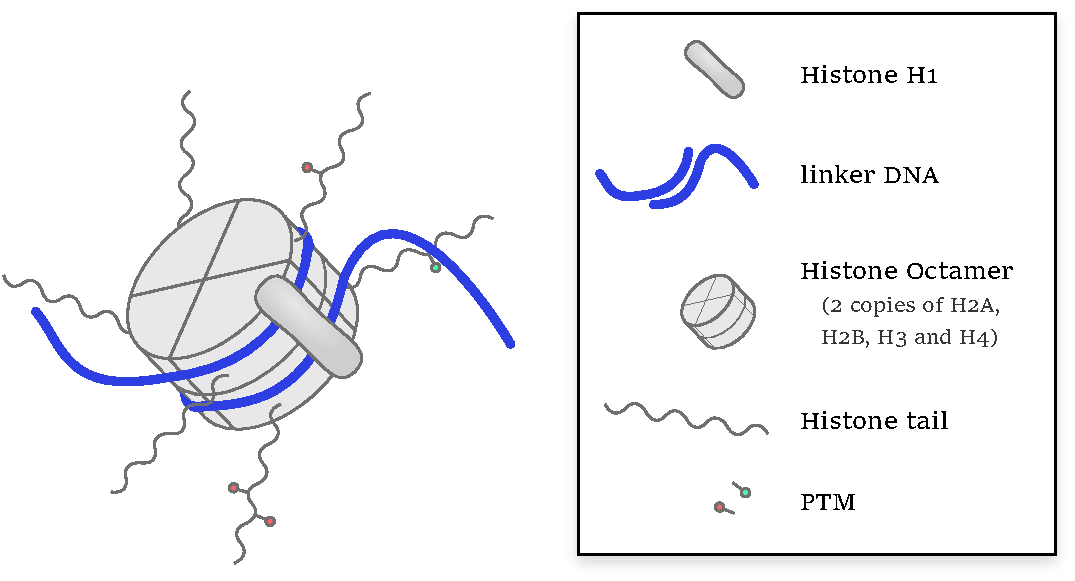
\includegraphics[width=0.7\textwidth]{annotated_nucleosome.pdf}
            \caption{Schematic model of a eukaryotic nucleosome. It consists of DNA wrapped around a histone octamer. The histones themselves are organized as one tetramer (two H3, two H4) and 2 homologous dimers (H2A, H2B). The DNA is kept in place by histone H1, which also plays a role in establishing higher order chromatin structures.}
            \label{img:nucleosome}
        \end{figure}
        %

        %
        Histones contain a great amount of the positively charged amino acids arginine (Arg, R) and lysine (Lys, K), which results in attracting the negatively charged DNA (phosphate backbone) \cite{berg2015stryer}.
        %

        %
        In Eukaryotic nucleosomes, the N-terminal amino acid tails stick out from the histone core complex (see model in fig. \ref{img:nucleosome}) and interact with tails from other nucleosomes and histone 1 (H1) (see fig. \ref{img:nucleosome}) to form higher-order chromatin structures which has a direct influence on transcriptional activity \cite{prohaska2010innovation}. The DNA's local availability as a protein binding site through these higher order structures is often expressed with the terms of open (or active) and closed (or silent) chromatin. However, given that, for instance, transcription factors (TFs) are able to open chromatin \cite{lomvardas2002opening}, it is important to point out the difference between the availability of chromatin and gene transcription activity. Nevertheless, ChAPs play an important role in a general gene activity machinery which is then, in most organisms, followed by more specific mechanisms as, for example, regulation through DNA-sequence-specific TF binding.
        %
    %
    %
    \section{Chemical histone modification}
        \label{subsec:HME}
        %
        Transcriptional regulation can mainly be achieved through two mechanisms \cite{prohaska2010innovation}: firstly by exchanging of ChAP variants \cite{henikoff2008nucleosome} and secondly by chemically modifying ChAPs.
        %


        %
        This thesis is based on one aspect of gene transcription regulation through chromatin (de)stabilization, namely the chemical modification by means of histone-modifying enzyme (HME) complexes. These complexes are able to covalently add or remove chemical groups on amino acids (mostly R and K) at very specific positions on the histone tail. These post-translational modifications (PTMs) are named according to the amino acid they have been bound to. H3K27ac, for instance, denotes an acetylation (\ac/) on lysine 27 (K27) of histone 3 (H3).
        %

        %
        Chemical ChAP modification was mainly observed in Archaea and Eukarya. In Archaea, chemical modification primarily serves the purpose of thermodynamically altering the chromatin's local stability \cite{henikoff2008nucleosome}.
        %

        %
        The presence of these chemical groups changes the charge or polarity of the modified amino acids and thus influences the histone's affinity to the DNA. Histone-acetyl\-transfer\-ases (HATs), for instance, add an acetyl group to lysine, thus neutralizing the positive charge on the ammonium cation at neutral pH (see figure \ref{img:acetyllysineReaction}). This neutralization decreases the attraction to the negatively charged DNA backbone significantly resulting in a more mobile nucleosome and, thus, more active chromatin \cite{berg2015stryer}.
        %

        %
        In Eukaryotes, additionally to the thermodynamic effect, modified histones can also be directly disassembled or evicted resulting in local histone depletion and more open chromatin \cite{henikoff2008nucleosome}.\\
        %

        %
        \begin{figure}[htpb]
            \centering
            \vspace{.5cm}
            \schemestart
                \arrow{0}[,0]
                \chemname{\chemfig{!{lysine}}}{Lysine}\+\chemname{\chemfig{!{acetylcoa}}}{Acetyl-CoA}
                \arrow[-90]
                \chemfig{!{acetyllysine}}\+\chemfig{CoA-SH}\+\chemfig{H^+}
            \schemestop
            \vspace{.5cm}
            \caption{Acetylation of lysine. This reaction is catalysed by the HAT enzyme which by means of the cofactor acetyl coenzyme A (Acetyl-CoA) is able to trigger the transfer (nucleophilic substitution reaction in chemical terms) of an acetyl group onto the nitrogen atom in the side chain of lysine. The latter can be part of a histone tail.}
            \label{img:acetyllysineReaction}
        \end{figure}
        %

        %
        Apart from the acetyl group, a multitude of other markers have been found on histone tails, e.g. methylation (one-, two and three-fold), phosphorylation, ubiquitylation and so forth \cite{bannister2011regulation}. These groups can entail gene transcription activation, silencing (repressing), or fulfil completely different purposes \cite{rossetto2012histone,wang2006histone}. For instance, phosphorylation cascades serve the purpose of rapidly responding to a potential health risk like heat shock \cite{prohaska2010innovation}. Mass-ubiquitination is thought to serve as markers in response to DNA damage resulting in its subsequent repair \cite{zhou2009histone}.\\
        %

        %
        The enzymes' modification activities are not forcibly isolated processes. The different enzyme types as well as the modifications on specific amino acids on the histone tails are connected through complex interaction networks \cite{zhang2015interplay, musselman2012perceiving, ge2019nucleation}. Such crosstalk between different modifications is achieved by the enzymes' ability to “read” modifications and “write” another one, if the reading process was successful. Reading is achieved by binding to specific modifications on the histone tail. A very popular example for such behaviour are enzymes presenting a bromodomain, which specifically binds acetylated lysines \cite{zeng2002bromodomain}. Upon successful binding, the enzyme can then catalyse the covalent modification of an unmodified amino acid. Additionally, proteins can also contain two bromodomains, thus reading two acetylation marks on two different nucleosomes which are arranged in a very specific topology to one another \cite{prohaska2010innovation}.
        %
    %
    %
    \section{Bivalency}
        %
        \label{sec:TheoryBivalency}
        In pluripotent stem cells, nucleosomes have been found to contain both activating and silencing markers on histone tails of one and the same octamer. This bivalent state is believed to maintain a “poised state”, being ready to induce a gene expression cascade as soon as the silencing marker is removed \cite{lesch2014poised,bernhart2016changes}.
        Others believe that this bivalent state is connected to cell division and the ability of inheriting the active gene set for one daughter cell to induce differentiation while the other daughter cell remains a pluripotent stem cell \cite{schuettengruber2017genome}.
        %

        %
        However, the notion of bivalency is not always reduced to one same nucleosome. It was also found that chromatin areas spanning over multiple nucleosomes showed presence of marks that are associated with gene transciption activation as well as silencing without the need of both modification types on one same nucleosome (see review \cite{Hoffmann2015BivalencyReview} for multiple examples). In proximity to genetic domains encoding developmental transcription factors, these poised areas are believed to function as \textit{epigenetic switches}, meaning that, once tilted in the “ON” or “OFF” direction, cell type specific gene activation or silencing can be heritably fixed \cite{Hoffmann2015BivalencyReview}. Thus, it can be argued that bivalent domains serve the purpose of reducing overall transcriptional noise \cite{Bernstein2006BivalentESC} while still keeping a certain degree of transcription willingness of the proximal gene.
        %
    %
    %
%
%